% Made up for the tikra benchmark.
% The phase diagram of water (a sketch, pressure on a log scale): ice, liquid and vapour, the
% triple point and the critical point.
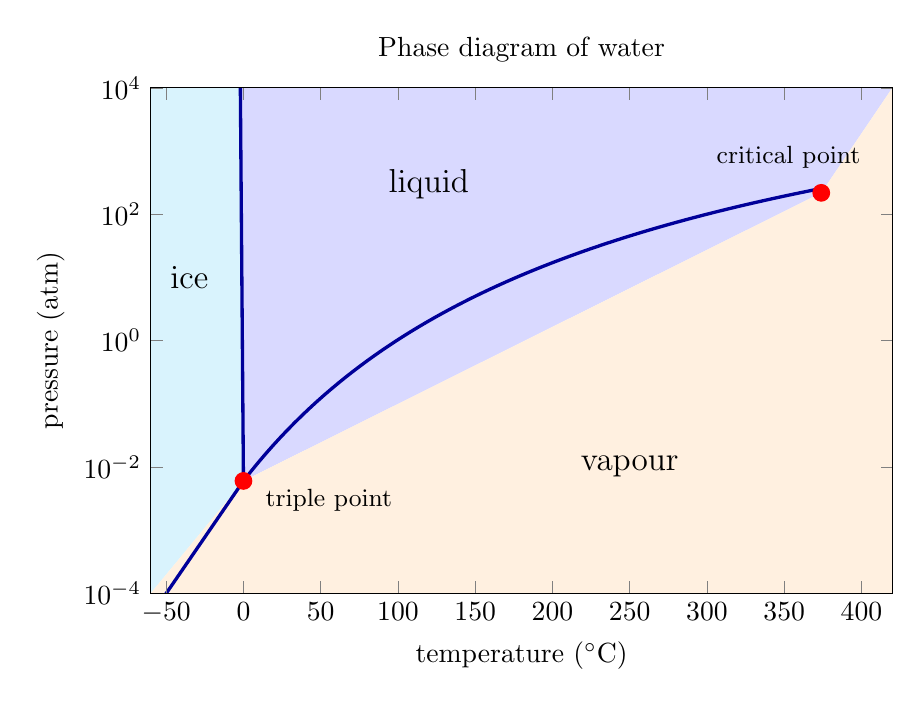
\begin{tikzpicture}
\begin{axis}[width=11cm, height=8cm, ymode=log, xmin=-60, xmax=420, ymin=1e-4, ymax=1e4,
    xlabel={temperature ($^\circ$C)}, ylabel={pressure (atm)}, title={Phase diagram of water},
    axis on top, ytick={1e-4,1e-2,1,1e2,1e4}]
  \fill[cyan!15] (axis cs:-60,1e-4) -- (axis cs:0.01,0.006) -- (axis cs:-2,1e4) -- (axis cs:-60,1e4) -- cycle;
  \fill[blue!15] (axis cs:0.01,0.006) -- (axis cs:374,218) -- (axis cs:420,1e4) -- (axis cs:-2,1e4) -- cycle;
  \fill[orange!12] (axis cs:-60,1e-4) -- (axis cs:0.01,0.006) -- (axis cs:374,218) -- (axis cs:420,1e4) -- (axis cs:420,1e-4) -- cycle;
  \addplot[very thick, blue!60!black, domain=-60:0.01, samples=40] {0.006*exp(0.082*x)};
  \addplot[very thick, blue!60!black, domain=0.01:374, samples=80] {0.006*exp(17.5*x/(x+240))*1.0} ;
  \addplot[very thick, blue!60!black] coordinates {(0.01,0.006) (-2,1e4)};
  \addplot[only marks, mark=*, mark size=3pt, red] coordinates {(0.01,0.006) (374,218)};
  \node[font=\large] at (axis cs:-35,10) {ice};
  \node[font=\large] at (axis cs:120,300) {liquid};
  \node[font=\large] at (axis cs:250,1e-2) {vapour};
  \node[font=\small, anchor=west] at (axis cs:8,0.003) {triple point};
  \node[font=\small, anchor=west] at (axis cs:300,800) {critical point};
\end{axis}
\end{tikzpicture}
